\documentclass[twocolumn, 10.5pt]{article}
\usepackage{verbatim}
\usepackage{amsfonts}
\usepackage{geometry}
\usepackage{amsmath}
\usepackage{amsthm}
\usepackage{amssymb}
\usepackage{listings}
\usepackage{graphicx}
\usepackage{clrscode3e}
\usepackage{txfonts}
\usepackage{fontspec}
%\usepackage{ctex}
\usepackage{float}
\usepackage{enumerate}
\setmainfont{Times New Roman}
\geometry{top=2.5cm,bottom=2.5cm,left=2.5cm,right=2.5cm}
\setlength\parindent{0em}
\begin{document}
	\title{Problem Solving Homework (Week 5)}\author{161180162 Xu Zhiming}\maketitle
	\section*{JH Chapter 3}
	\subsection*{3.6.1.3}
	\begin{proof}
		According to the definition, we can verify the following three conditions:
		\begin{enumerate}
			\item Suppose $\alpha\in M(x)$, then $\alpha\in f_x(\alpha)$ because, if we flip no variable in $\alpha$, $\alpha$ is mapped to itself
			\item $\alpha\in M(x)$ and $\beta\in f_x(\alpha)$. Then we have $\alpha$ and $\beta$ have at most one variable that is not the same. If $\alpha=\beta$, from 1. we have $\alpha\in f_x(\beta)$. If they are not the same, flipping the only different variable will transform $\alpha$ to $\beta$, therefore, $\alpha\in f_x(\beta)$ 
			\item $k$ can be the number of all variables in \proc{Max-Sat}, $\gamma_1$ and $\alpha$ have one different variable. $\gamma_k$ and $\beta$ have one different variable. $\gamma_i$ and $\gamma_{i+1}$ have one different variable for $i=1,2,\cdots,k-1$. These assignments satisfy the definition.
			\end{enumerate}
	\end{proof}
	\section*{TSP}
	\subsection*{2-exchange}
	\begin{proof}
		The following graph servers as a counterexample. If the original solution is $\{1,2,3,4,5,1\}$, 2-exchange will never lead to $\{1,3,5,2,4,1\}$, which is optimal.
		\begin{figure}[H]
			\centering
			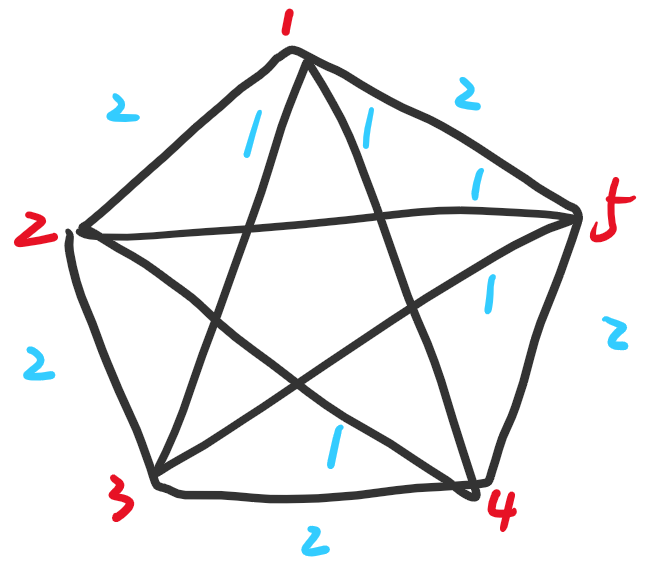
\includegraphics[width=0.7\linewidth]{ex5-1}
		\end{figure}
	\end{proof}
	\subsection*{(n-1)-exchange}
	\begin{proof} 
		The former graph can also serve as a counterexample, i.e., (n-1)-exchange is still not accurate, which means the problem itself is wrong.
	\end{proof}
	\section*{Accurate local search}
	\begin{enumerate}[(1)]
		\item No, it is not accurate.\\
		Suppose the cut generated by this algorithm is $S$. Let $v$ be a vertex in $S$. Consider the set $E_v$ of edges incident to $v$. If we move $v$ from $S$ to $S'=V\backslash S$ Since $S$ is a local optimum, moving $v$ to $S'$ does not increase the cut value. Therefore:
		\[
		\begin{aligned}
			\sum_{u\in S',(u,v)\in E}w_{u,v}\ge \sum_{u\in S',(u,v)\in E}w_{u,v}\\
			2\sum_{u\in S',(u,v)\in E}w_{u,v}\ge \sum_{u\in S',(u,v)\in E}w_{u,v}+\sum_{u\in S',(u,v)\in E}w_{u,v}\\
			\sum_{u\in S',(u,v)\in E}w_{u,v}\ge \frac{1}{2}\sum_{u:(u,v)\in E}w_{u,v}\\
			\sum_{u\in S,(u,v')\in E}w_{u,v'}\ge \frac{1}{2}\sum_{u:(u,v')\in E}w_{u,v}\\
			\therefore 2c(S)=2\sum_{u\in S,v\in S',(u,v)\in E}w_{u,v}\ge \sum_{e\in E}w_e\ge OPT
		\end{aligned}
		\]
		That is, this algorithm generates a solution that is no smaller than half the optimal one(s).
		\item The worst case time complexity is exponential.
	\end{enumerate}
\end{document}